% This file was created by tikzplotlib v0.9.8.
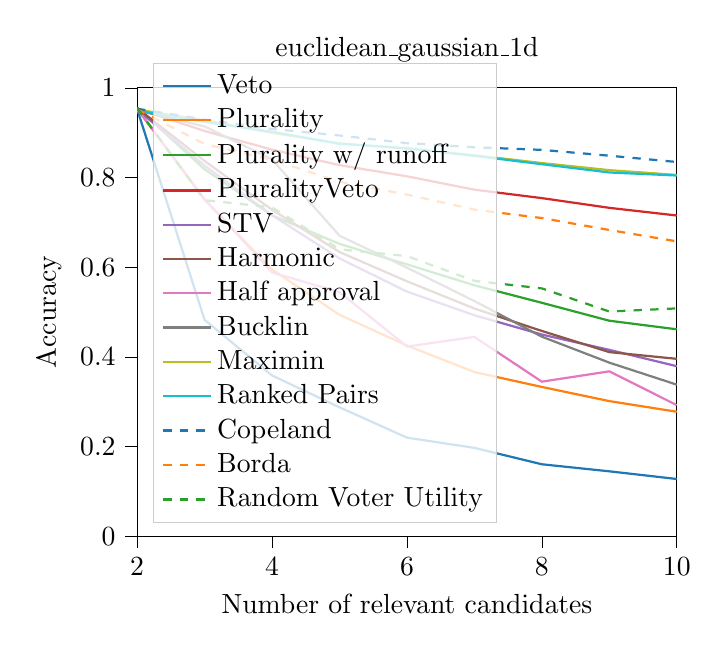
\begin{tikzpicture}

\definecolor{color0}{rgb}{0.12156862745098,0.466666666666667,0.705882352941177}
\definecolor{color1}{rgb}{1,0.498039215686275,0.0549019607843137}
\definecolor{color2}{rgb}{0.172549019607843,0.627450980392157,0.172549019607843}
\definecolor{color3}{rgb}{0.83921568627451,0.152941176470588,0.156862745098039}
\definecolor{color4}{rgb}{0.580392156862745,0.403921568627451,0.741176470588235}
\definecolor{color5}{rgb}{0.549019607843137,0.337254901960784,0.294117647058824}
\definecolor{color6}{rgb}{0.890196078431372,0.466666666666667,0.76078431372549}
\definecolor{color7}{rgb}{0.737254901960784,0.741176470588235,0.133333333333333}
\definecolor{color8}{rgb}{0.0901960784313725,0.745098039215686,0.811764705882353}

\begin{axis}[
legend cell align={left},
legend style={
  fill opacity=0.8,
  draw opacity=1,
  text opacity=1,
  at={(0.03,0.03)},
  anchor=south west,
  draw=white!80!black
},
tick align=outside,
tick pos=left,
title={euclidean\_gaussian\_1d},
x grid style={white!69.0196078431373!black},
xlabel={Number of relevant candidates},
xmin=2, xmax=10,
xtick style={color=black},
y grid style={white!69.0196078431373!black},
ylabel={Accuracy},
ymin=0, ymax=1,
ytick style={color=black}
]
\addplot [thick, color0]
table {%
2 0.9526
3 0.4825
4 0.3585
5 0.2875
6 0.2198
7 0.197
8 0.1604
9 0.1447
10 0.1276
};
\addlegendentry{Veto}
\addplot [thick, color1]
table {%
2 0.9535
3 0.7503
4 0.5949
5 0.4938
6 0.4253
7 0.3661
8 0.3329
9 0.3013
10 0.2776
};
\addlegendentry{Plurality}
\addplot [thick, color2]
table {%
2 0.9561
3 0.8184
4 0.7157
5 0.6519
6 0.6063
7 0.5596
8 0.5206
9 0.4806
10 0.4615
};
\addlegendentry{Plurality w/ runoff}
\addplot [thick, color3]
table {%
2 0.9537
3 0.9038
4 0.8622
5 0.8276
6 0.8027
7 0.7729
8 0.7541
9 0.7324
10 0.7153
};
\addlegendentry{PluralityVeto}
\addplot [thick, color4]
table {%
2 0.952
3 0.8266
4 0.7158
5 0.6197
6 0.5456
7 0.4928
8 0.4498
9 0.4156
10 0.3792
};
\addlegendentry{STV}
\addplot [thick, color5]
table {%
2 0.9549
3 0.837
4 0.7281
5 0.6338
6 0.5686
7 0.5078
8 0.4578
9 0.4106
10 0.3956
};
\addlegendentry{Harmonic}
\addplot [thick, color6]
table {%
2 0.9535
3 0.7522
4 0.5883
5 0.5443
6 0.4231
7 0.4445
8 0.3447
9 0.3677
10 0.2923
};
\addlegendentry{Half approval}
\addplot [thick, white!49.8039215686275!black]
table {%
2 0.9502
3 0.914
4 0.8405
5 0.6702
6 0.599
7 0.5245
8 0.445
9 0.3871
10 0.338
};
\addlegendentry{Bucklin}
\addplot [thick, color7]
table {%
2 0.9516
3 0.9277
4 0.8996
5 0.8762
6 0.8643
7 0.8498
8 0.8323
9 0.8165
10 0.8058
};
\addlegendentry{Maximin}
\addplot [thick, color8]
table {%
2 0.949
3 0.9241
4 0.9021
5 0.8753
6 0.8655
7 0.8483
8 0.8297
9 0.8113
10 0.8045
};
\addlegendentry{Ranked Pairs}
\addplot [thick, color0, dashed]
table {%
2 0.9534
3 0.9293
4 0.9083
5 0.8938
6 0.8767
7 0.8675
8 0.8617
9 0.8487
10 0.8347
};
\addlegendentry{Copeland}
\addplot [thick, color1, dashed]
table {%
2 0.9522
3 0.8747
4 0.8397
5 0.7907
6 0.762
7 0.7285
8 0.7096
9 0.683
10 0.6576
};
\addlegendentry{Borda}
\addplot [thick, color2, dashed]
table {%
2 0.9547
3 0.7495
4 0.7336
5 0.6399
6 0.6249
7 0.5695
8 0.5527
9 0.5011
10 0.5081
};
\addlegendentry{Random Voter Utility}
\end{axis}

\end{tikzpicture}
